\documentclass[a4paper,12pt]{article} % добавить leqno в [] для нумерации слева
\usepackage[a4paper,top=1.3cm,bottom=2cm,left=1.5cm,right=1.5cm,marginparwidth=0.75cm]{geometry}
%%% Работа с русским языком
\usepackage{cmap}					% поиск в PDF
\usepackage[warn]{mathtext} 		% русские буквы в фомулах
\usepackage[T2A]{fontenc}			% кодировка
\usepackage[utf8]{inputenc}			% кодировка исходного текста
\usepackage[english,russian]{babel}	% локализация и переносы
\usepackage{physics}
\usepackage{multirow}
\usepackage{longtable}

%%% Нормальное размещение таблиц (писать [H] в окружении таблицы)
\usepackage{float}
\restylefloat{table}

\usepackage{graphicx}
\usepackage{subcaption}
\usepackage[]{float}
\usepackage{graphicx}

\usepackage{wrapfig}
\usepackage{tabularx}

\usepackage{hyperref}
\usepackage[rgb]{xcolor}
\hypersetup{
	colorlinks=true,urlcolor=blue
}

\usepackage{pgfplots}
\pgfplotsset{compat=1.9}

%%% Дополнительная работа с математикой
\usepackage{amsmath,amsfonts,amssymb,amsthm,mathtools} % AMS
\usepackage{icomma} % "Умная" запятая: $0,2$ --- число, $0, 2$ --- перечисление

%% Номера формул
\mathtoolsset{showonlyrefs=true} % Показывать номера только у тех формул, на которые есть \eqref{} в тексте.

%% Шрифты
\usepackage{euscript}	 % Шрифт Евклид
\usepackage{mathrsfs} % Красивый матшрифт

%% Свои команды
\DeclareMathOperator{\sgn}{\mathop{sgn}}

%% Перенос знаков в формулах (по Львовскому)
\newcommand*{\hm}[1]{#1\nobreak\discretionary{}
	{\hbox{$\mathsurround=0pt #1$}}{}}

\date{\today}

\usepackage{gensymb}
f
\title{Лабораторная работа 2.3.1 : Получение и измерение вакуума}
\author{Сидорчук Максим Б01-204}
\date{\today}
\begin{document}
\maketitle

\section{Теоретические сведения}
Производительность насоса определяется скоростью откачки W (л/с): W -- это объём газа, удаляемого из сосуда при заданном давлении за единицу времени. Скорость откачки форвакуумного насоса равна ёмкости воздухозаборной камеры, умноженной на число оборотов в секунду.

Обозначим количество газа, которое приходит в трубку в процессе откачки за \(Q\). Тогда мы можем записать уравнение:
\[-VdP = (PW - Q)dt\]

Но при предельном давлении \(\frac{dP}{dt} = 0 \Rightarrow Q = P_{пр}W\). Подставим это в начальное уравнение и проинтегрируем. Учитывая, что \(P_0 \gg P_{пр}\):
\[
    P - P_{\text{пр}} = P_0 e^{-Wt/V}
\]
Постоянная времени откачки $\tau = V/W$ является мерой эффективности откачанной системы.
Для течения газа через трубу при высоком вакууме справедлива формула:
\[\frac{d(PV)}{dt} = \frac{4}{3}r^3\sqrt{\frac{2\pi RT}{\mu}} \frac{P_2 - P_1}{L}\]
Если пренебречь давлением $P_1$ у конца, обращенного к насосу, получаем формулу для пропускной способности трубы:
\[C_{тр} = \frac{dV}{dt} = \frac{4}{3}\frac{r^3}{L}\sqrt{\frac{2\pi RT}{\mu}}\]
Для пропускной способности отверстия (например в кранах) имеем формулу:
\[C_{отв}=S\frac{\bar v}{4}\]

\section{Экспериментальная установка}

Установка изготовлена из стекла и состоит из форвакуумного баллона (ФБ), высоковакуумного диффузионного насоса (ВН), высоковакуумного баллона (ВБ), масляного (М) и ионизационного (И) манометров, термопарных манометров (М$_1$ и М$_2$), форвакуумного насоса (ФН) и соединительных кранов (Рис. \ref{ris:ustanovka}). Кроме того, в состав установки входят: вариатор (автотрансформатор с регулируемым выходным напряжением), или реостат и амперметр для регулирования тока нагревателя диффузионного насоса.
\begin{figure}[H]
    \center{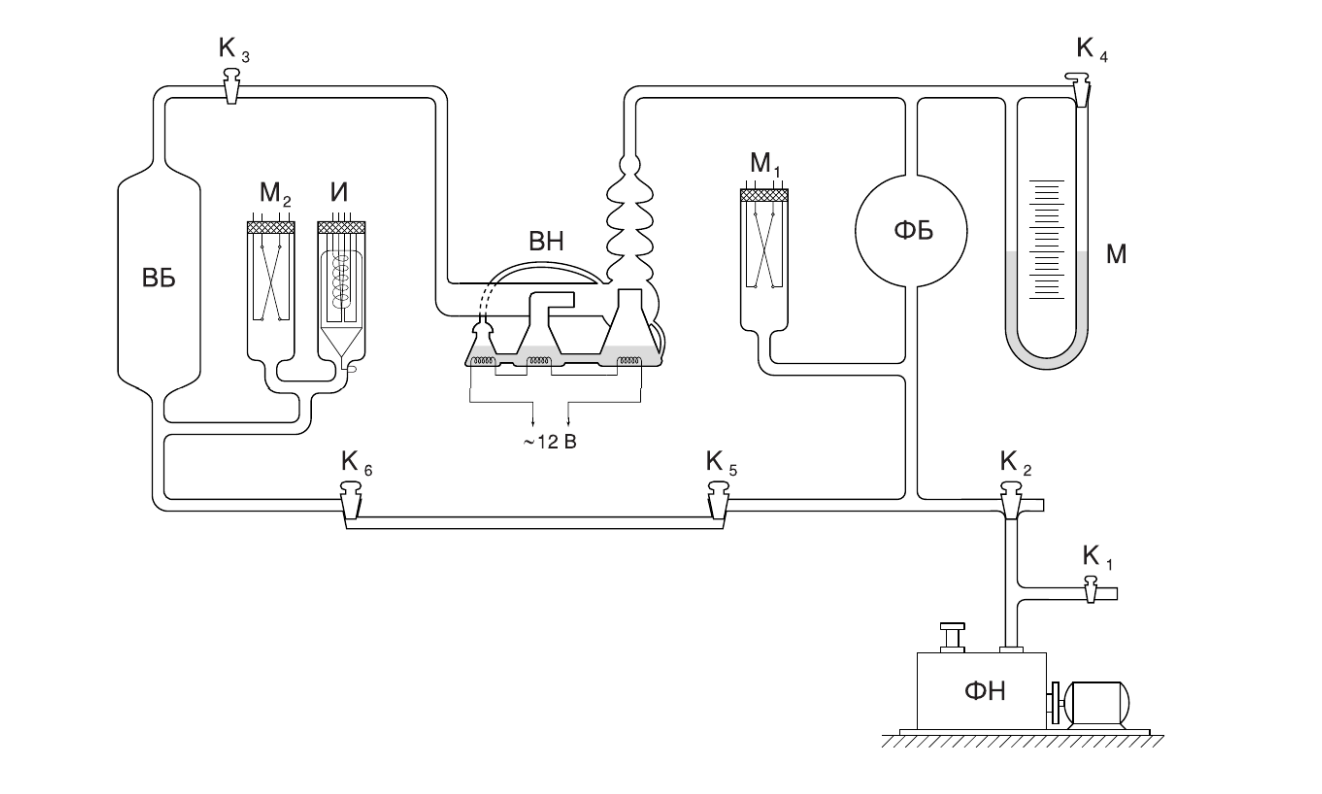
\includegraphics[width=0.8\textwidth]{ustanovka.png}}
    \caption{Схема экспериментальной установки.}
    \label{ris:ustanovka}
\end{figure}

\section{Ход работы}

\subsection*{Измерение объёмов форвакуумной и высоковакуумной частей установки}
	\begin{enumerate}
		\item Проверяем, что $K_4$ открыт, впускаем в установку атмосферный воздух через краны $K_1$ и $K_2$. <<Запираем>> в капилляре атмосферный воздух кранами $K_5$ и $K_6$. Объем капилляра в используемой установке: $$V_\text{к} = 50~ \text{см}^3.$$
		\item Закрываем $K_1$ и $K_2$, включаем форвакуумный насос и даём ему откачать себя. Подключаем установку к насосу краном $K_2$. Откачиваем установку до $10^{-2}$ торр. Отсоединяем установку краном $K_2$, и оставляем насос работать <<на себя>>. Перекрываем  $K_3$, отделяя высоковакуумною часть установки. Закрываем  $K_4$, чтобы привести в готовность масляный манометр.
		\item Открываем  $K_5$, чтобы <<запертый>> ранее воздух заполнил форвакуумную часть установки, снимаем давление с помощью вакуумного манометра, измерив разность высот столбиков масла (приводим результаты и повторного измерения):
		$$
		\Delta h_1 = (26.2\pm0.1) ~\text{мм};
		$$
		Погрешность измерения величин определяется ценой деления шкалы манометра и способностью разглядеть показания.
		\item Имея в виду, что плотность масла в манометре равна 885 г/л, и считая, что установившееся давление много больше форвакуумного, получаем:
		$$
		P_1 = (2.31\pm0.01)~\text{Па};
		$$
		Пользуясь законом Бойля-Мариотта (т.к. расширение газа изотермическое), используя среднее значение измеренного давления, получаем
		$$
		V_\text{ФВ} = (2.18\pm0.02)~\text{л}
		$$
		\item Аналогично, открыв кран $K_3$, получив значения разности высот на манометре, получаем объем высоковакуумной части установки:
		$$
		V_\text{ВВ} = (1.28\pm0.06)~\text{см}^3
		$$
            \item Тогда общий объём установки равен (погрешности складываются):
            $$
		V_\Sigma = (3.46\pm0.08)~\text{см}^3
		$$
		\item Открываем кран $K_4$.
	\end{enumerate}

 \subsection*{Получение высокого вакуума}
	\begin{enumerate}
	\item Откачиваем установку ФВ насосом.
	\item Включаем термопарные манометры, устанавливаем их токи согласно паспортам. Переключаем прибор в режим измерения ЭДС и определяем давление в установке по градуировочной кривой
	\item По достижении форвакуума закрываем $K_5$ и начинаем откачку высоковакуумного баллона с помощью диффузионного насоса, для этого:\\
	3.1. На передней панели источника питания, с помощью которого подогревается масло в насосе, все четыре ручки переводим на ноль.\\
	3.2. Включаем источник, ручками 2 и 4 устанавливаем ток $I = 0.6A$. Ждём 5 минут, чтобы масло прогрелось, после чего устанавливаем ток $1.15A$. \\
	3.3. По термопаре $M_2$ контролируем откачку. По достижении ЭДС в 10mV смотрим на кипение масла и считаем капли, стекающие из сопла второй ступени. Убеждаемся в готовности, т.к. насчитали 11 капель в минуту.
	\item При выключенной ионизационной лампе, вставив предохранитель, ставим переключатель <<Род работы>> в положение <<Обезгаживание>> на 10 минут.
	\item Переключатель <<Множитель шкалы>> ставим в положение <<Установка нуля>>, <<Род работы>> в положение <<Установка эмиссии>>, и ручку <<Установка эмиссии>> ставим в крайнее левое положение.
	\item Приступаем к включению ионизационной лампы.
	\item Измеряем давление с помощью микроамперметра. Так как переключатель <<Множитель шкалы>> в положении $10^{-1}$, а постоянная ионизационного манометра $С = 100$ мм.рт.ст., то давление будет определяться как $P = 10^{-5}\cdot I$, где I -- показания микроамперметра в делениях. \\
	$$P_{\text{пр}} = 0.83\cdot10^{-4} ~\text{торр}$$
\end{enumerate}

\subsection*{Измерение скорости по ухудшению и улучшению вакуума}

\begin{center}
    \begin{table}
        \begin{tabular}{|c|c|c|c|c|c|c|c|c|c|}
            \hline
            \multicolumn{2}{|c|}{\textbf{Ухудшение 1}} & \multicolumn{2}{|c|}{\textbf{Ухудшение 2}} & \multicolumn{2}{|c|}{\textbf{Ухудение 3}} & \multicolumn{2}{|c|}{\textbf{Улучшение 1}} & \multicolumn{2}{|c|}{\textbf{Улучшение 2}} \\\hline
            \textbf{$10^{-4}$, торр}               & \textbf{t, c}                              & \textbf{$10^{-4}$, торр}              & \textbf{t, c}                              & \textbf{$10^{-4}$, торр} & \textbf{t, c} & \textbf{$10^{-4}$, торр} & \textbf{t, c} & \textbf{$10^{-4}$, торр} & \textbf{t, c} \\ \hline
            0.54                                       & 0                                          & 0.33                                      & 0                                          & 0.37                         & 0             & 6.0                          & 0.0           &  8.6  & 0.0   \\ \hline
            0.82                                       & 5                                          & 0.54                                      & 5                                          & 0.41                         & 5             & 5.8                          & 0.16          &  8.2  & 0.16  \\ \hline
            1.3                                        & 10                                         & 0.73                                      & 10                                         & 0.58                         & 10            & 5.5                          & 0.33          &  7.7  & 0.33  \\ \hline
            2.1                                        & 15                                         & 0.89                                      & 15                                         & 0.76                         & 15            & 5.4                          & 0.5           &  6.6  & 0.5   \\ \hline
            2.4                                        & 20                                         & 1.1                                       & 20                                         & 0.93                         & 20            & 5.2                          & 0.75          &  5.5  & 0.75  \\ \hline
            2.9                                        & 25                                         & 1.2                                       & 25                                         & 1.1                          & 25            & 5.0                          & 1             &  4.3  & 1     \\ \hline
            3.2                                        & 30                                         & 1.4                                       & 30                                         & 1.2                          & 30            & 4.7                          & 1.25          &  3.5  & 1.25  \\ \hline
            3.6                                        & 35                                         & 1.5                                       & 35                                         & 1.4                          & 35            & 4.3                          & 1.5           &  3.0  & 1.5   \\ \hline
            4.0                                        & 40                                         & 1.7                                       & 40                                         & 1.6                          & 40            & 4.0                          & 2             &  2.6  & 2     \\ \hline
            4.3                                        & 45                                         & 1.8                                       & 45                                         & 1.8                          & 45            & 3.2                          & 3             &  2.3  & 3     \\ \hline
            4.7                                        & 50                                         & 2.0                                       & 50                                         & 1.9                          & 50            & 2.7                          & 4             &  2.0  & 4     \\ \hline
            5.0                                        & 55                                         & 2.2                                       & 55                                         & 2.2                          & 55            & 2.0                          & 6             &  1.6  & 6     \\ \hline
            5.5                                        & 60                                         & 2.4                                       & 60                                         & 2.3                          & 60            & 1.5                          & 9             &  1.2  & 9     \\ \hline
            5.8                                        & 65                                         & 2.5                                       & 65                                         & 2.5                          & 65            & 1.2                          & 12            &  0.9  & 12    \\ \hline
            6.0                                        & 70                                         & 2.6                                       & 70                                         & 2.6                          & 70            & 0.9                          & 15            &  0.8  & 15    \\ \hline
        \end{tabular}
    \end{table}
\end{center}
\begin{enumerate}
    \item Закрываем кран $K_3$, отключая тем самым откачку вакуума и записываем на видео изменения показаний микроамперметра, пока вакуум не ухудшится до $6\cdot10^{-4}$ торр. Затем открываем $K_3$ и так же записываем улучшение вакуума. Приводим результаты повторных измерений в таблице 1 и на графиках (рис. 2, 3 и 4).

    \begin{figure}[H]
        \centering
        \begin{subfigure}[b]{0.4\textwidth}
          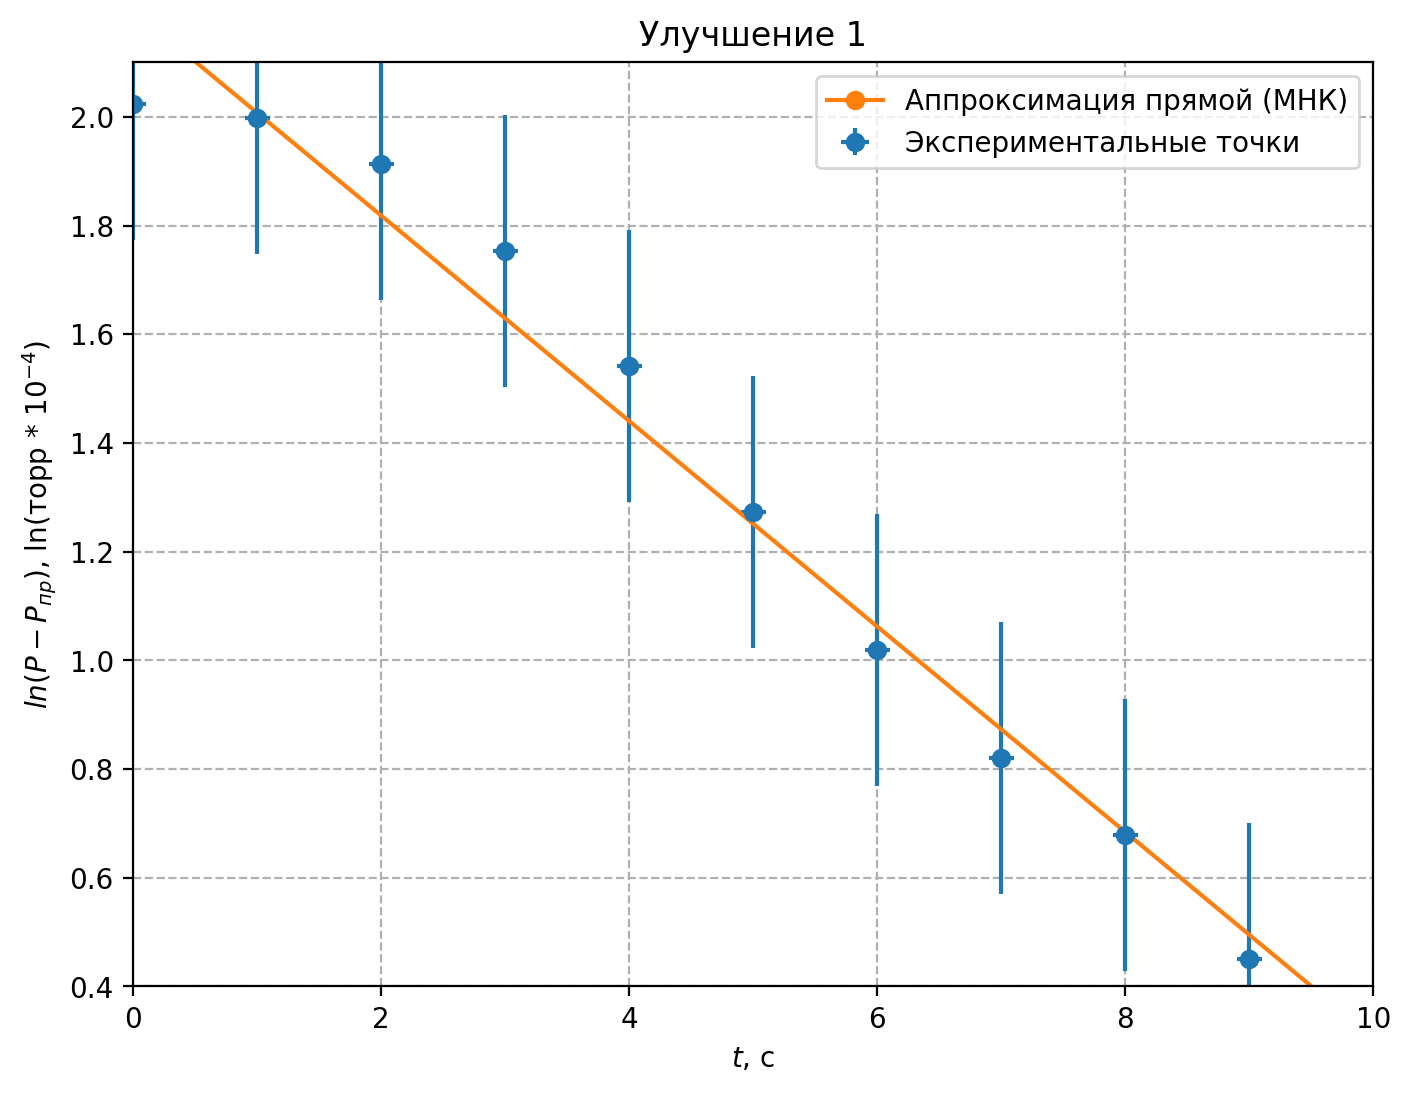
\includegraphics[width=\textwidth]{graphdown1.png}
        \end{subfigure}
        \hfill
        \begin{subfigure}[b]{0.4\textwidth}
          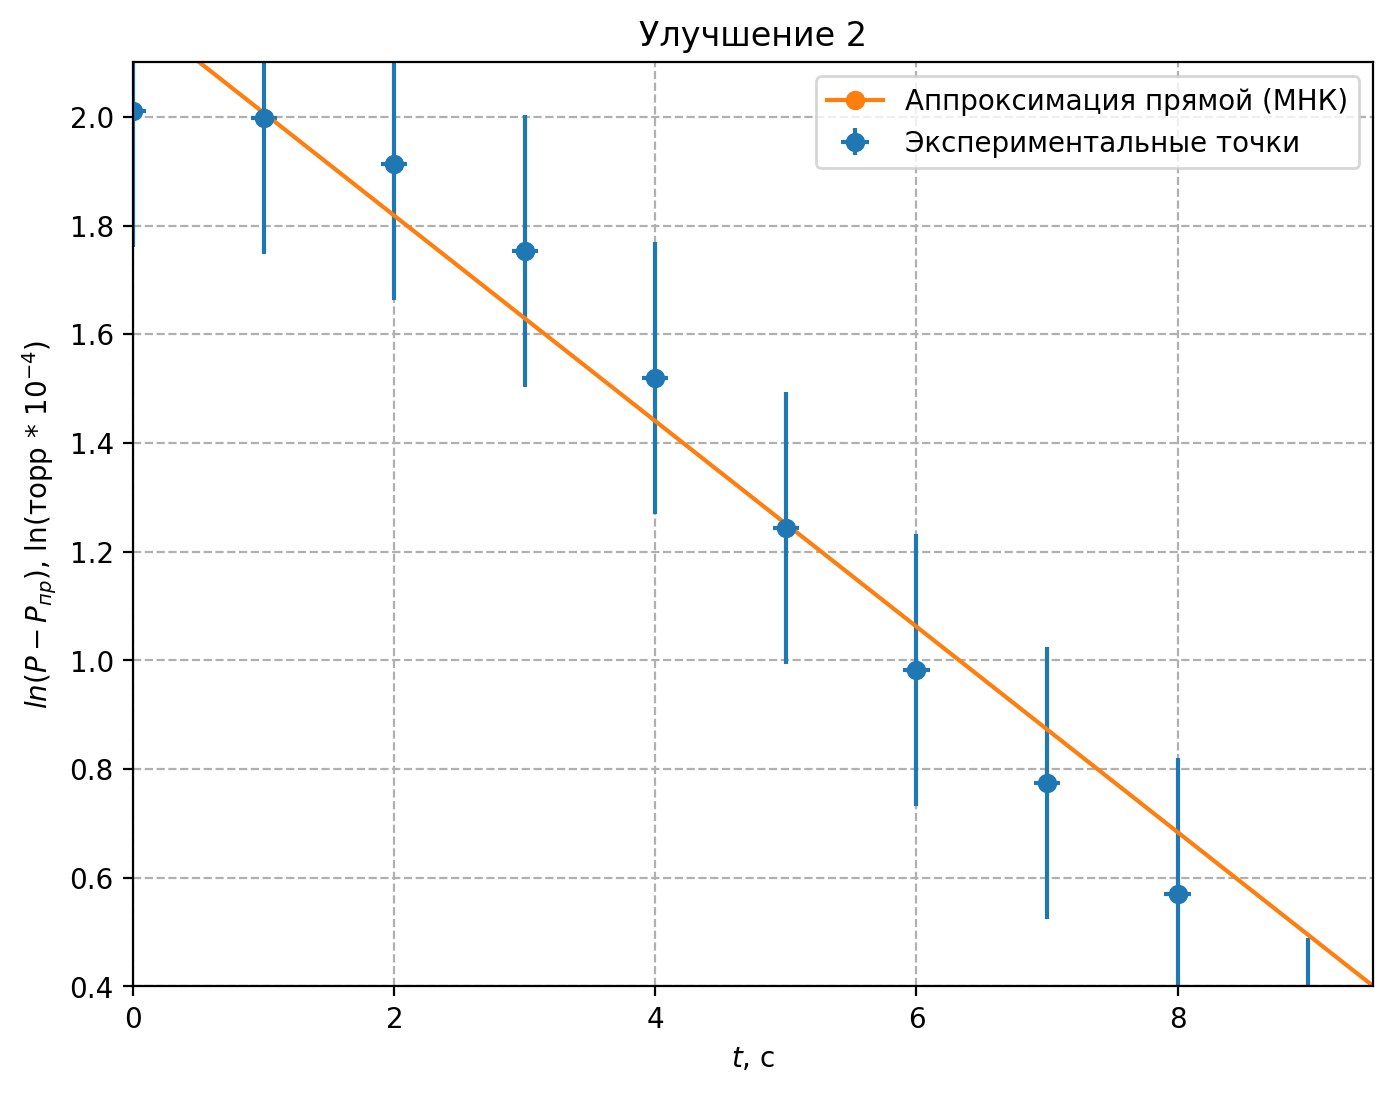
\includegraphics[width=\textwidth]{graphdown2.png}
        \end{subfigure}
        \caption{Зависимость $ln(P-P_{\text{пр}})$ от времени по улучшении вакуума.}
      \end{figure}
      \begin{figure}[H]
        \centering
        \begin{subfigure}[b]{0.4\textwidth}
          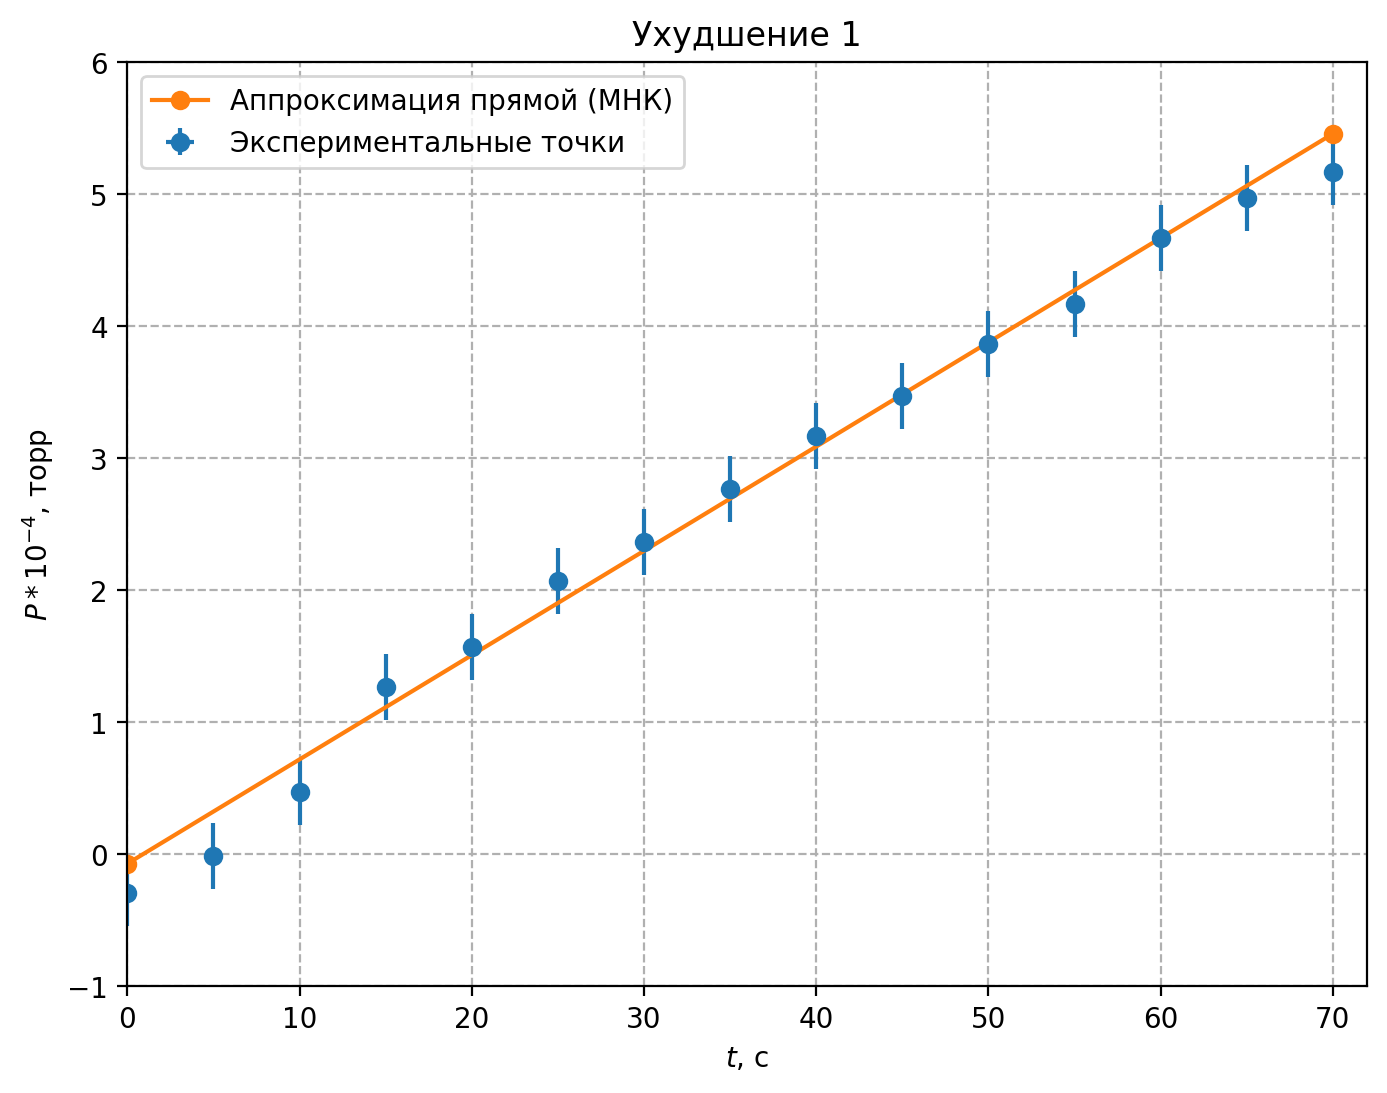
\includegraphics[width=\textwidth]{graphup1.png}
        \end{subfigure}
        \hfill
        \begin{subfigure}[b]{0.4\textwidth}
          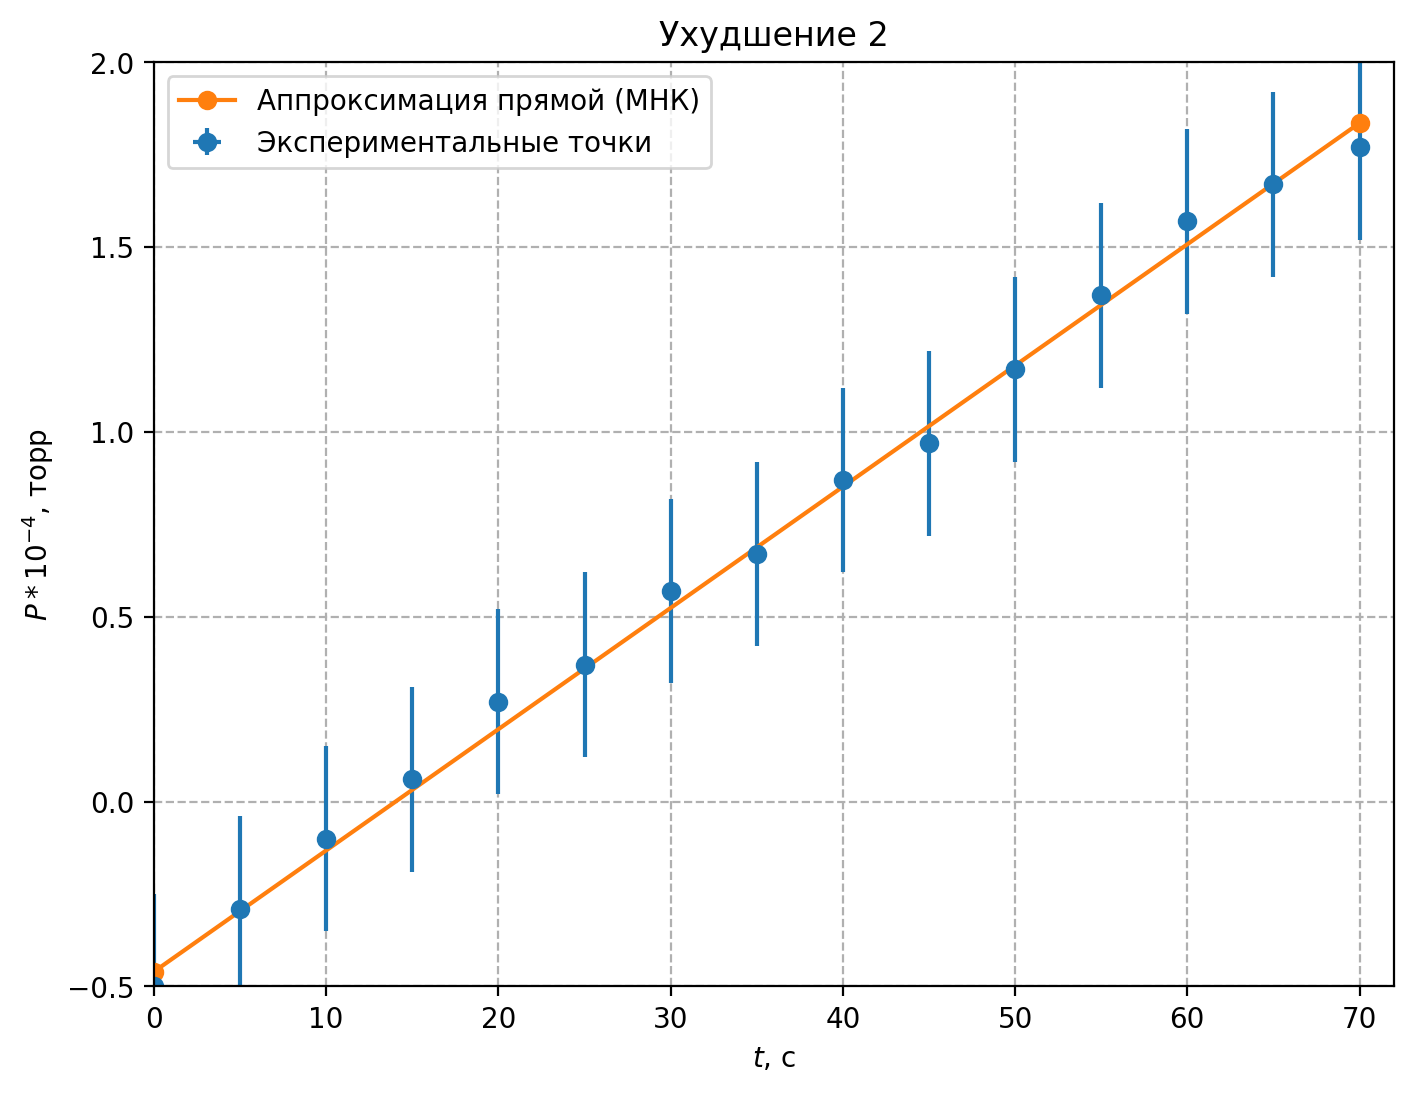
\includegraphics[width=\textwidth]{graphup2.png}
        \end{subfigure}
        \caption{Зависимость давления от времени по ухудшению вакуума.}
      \end{figure}
        \begin{figure}[H]
            \center{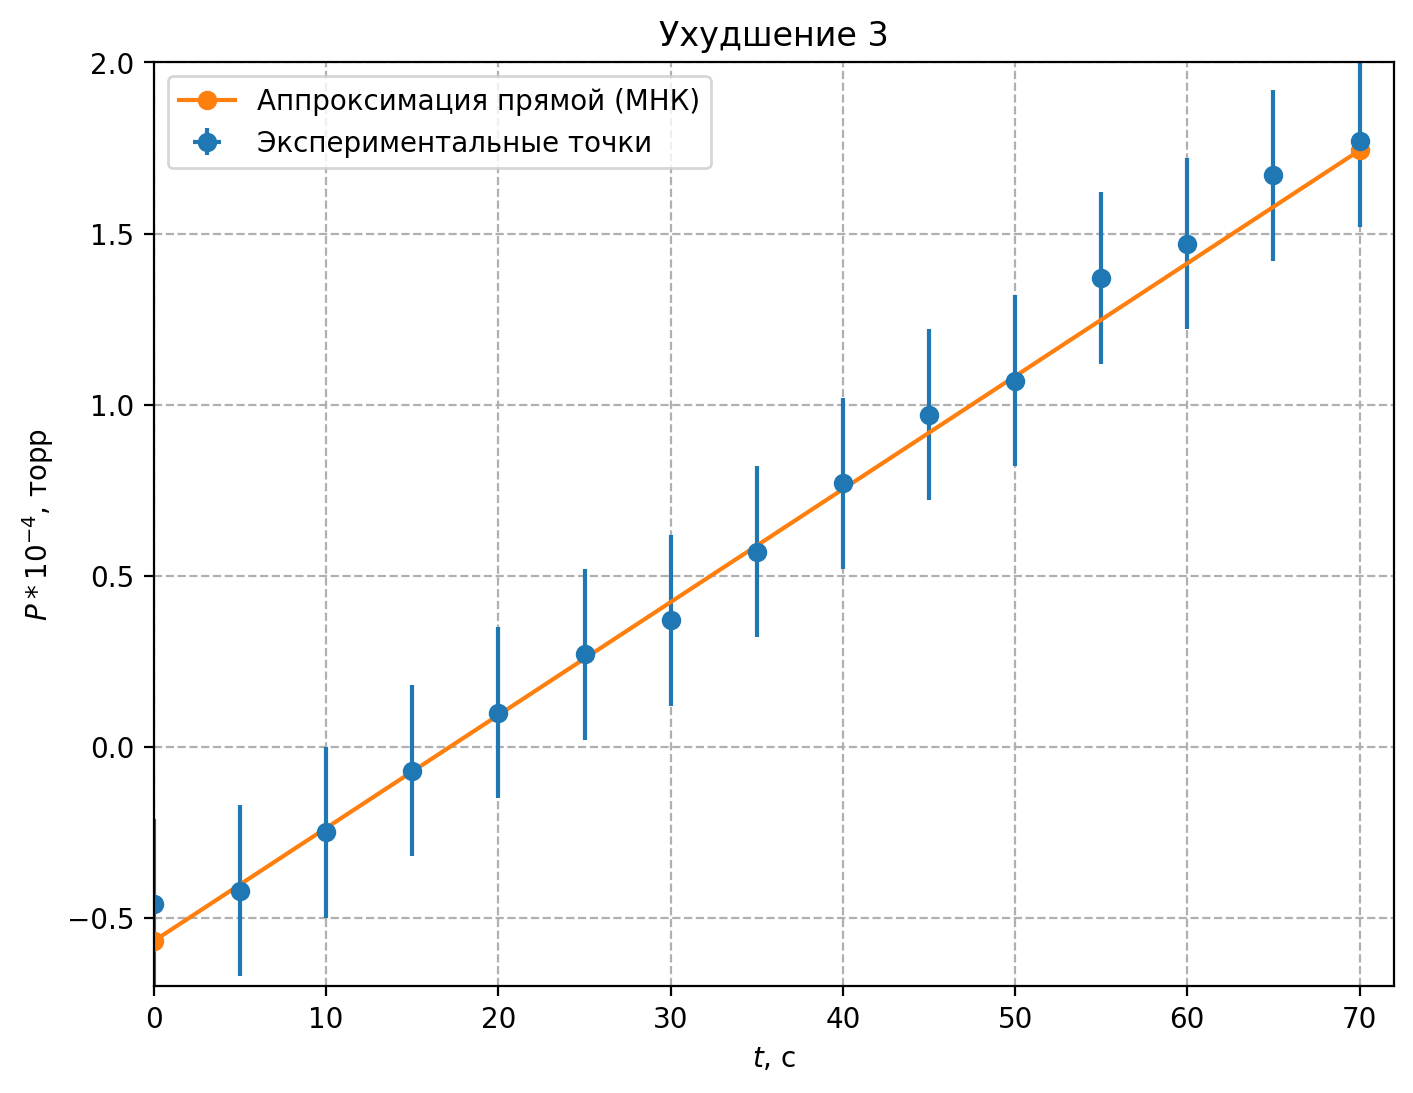
\includegraphics[width=0.45\textwidth]{graphup3.png}}
            \caption{Зависимость давления от времени по ухудшению вакуума.}
        \end{figure}

    \item
          Рассчитав коэффициенты наклона графиков 2(а) и 2(б) и зная объем высоковакуумной части установки, получим скорость откачки W диффузионного насоса, сравнив графики с зависимостью (4). Считаем $$W = -\bar{a}\cdot V, \quad\varepsilon_W^2 = \varepsilon_{\bar{a}}^2 + \varepsilon_V^2$$,  где $\bar{a}$ --- среднее коэффициентов наклона из зависимостей 2(а) и 2(б). Имеем:
          $$W = (0.461\pm0.016) ~\text{л/с}$$
    \item
          Имея в виду соотношения (1) для случая ухудшения вакуума (без откачки), оценим $Q_\text{н}$ c помощью полученных зависимостей 3(а, б) и 4. Считаем $$\frac{dP}{dt} = \bar{a}$$ где $\bar{a}$ --- среднее коэффициентов наклона из зависимостей 3 (а, б) и 4. Имеем:
          $$Q_\text{н} + Q_\text{д} = (1.26\pm0.04)\cdot 10^{-5} ~\text{торр}\cdot\text{л/c}$$
          $Q_\text{д}$ обычно порядка $10^{-8}$, поэтому можно считать $Q_\text{н} + Q_\text{д} \approx Q_\text{н}$. Таким образом,
          $$Q_\text{н} + Q_\text{д} \approx 1.26\cdot 10^{-5} ~\text{торр}\cdot\text{л/c}$$
    \item Оценим пропускную способность трубы от вакуумного баллона, имея в виду порядки её диаметра и длины и размерного множителя $$d \sim 10^{-2}~\text{м},\quad L \sim 1 ~\text{м},\quad \sqrt{\frac{RT}{\mu}} \sim 500 ~\text{м/с},$$ используя формулу (6) имеем:
          $$C_\text{тр} \sim 1 ~\text{л/с},$$
          что отлично согласуется с полученным ранее значением W.
    \item
          Рассчитаем производительность насоса ещё одним способом: создав искусственную течь. Открываем кран $K_6$ при включённом  насосе и измеряем давление, установившееся при течи. Оно равно $$P_\text{уст} = 1.9 \cdot 10^{-4} ~\text{торр}.$$
          Запишем (2) для данного случая:
          $$P_\text{пр}W = Q_1, \quad P_\text{уст}W = Q_1 + \frac{(PV)_\text{капилляр}}{dt}$$
          С учётом (6) получаем
          $$(P_\text{уст} - P_\text{пр})W = \frac{4}{3}(d/2)^3\sqrt{\frac{2\pi RT}{\mu}}\frac{P_\text{фв}}{L},$$
          где d и L --- диаметр и длина капилляра, равные
          $$d = 9 ~\text{мм},\quad L = 63 ~\text{мм}$$
          Получаем:
          $$W = 0.38 ~\text{л/c}$$
\end{enumerate}

\section{Вывод}
В данной работе была измерена производительность насоса с точностью $\epsilon = 0.03$, проверены теоретические зависимости, связанные с течением газа (рис. 2, 3 и 4). Было вычисленно предельное значение давления $P_{\text{пр}} = 0.83 \cdot 10^{-4}$ торр, а также скорость откачки, среднее значение которой равно $W_{ср} \approx 0.43$ л/с.

\end{document}


\end{document}